\documentclass[conference,harvard,brazil,english]{sbatex}
\usepackage[utf8]{inputenc}
\usepackage{lmodern}
\usepackage{amsmath}
\usepackage{graphicx}
\usepackage{float}

\begin{document}

\title{Controle de Temperatura de uma Torneira Elétrica}

% authors only; addresses and emails have been removed from the class
\author{Eduardo Henrique Basilio de Carvalho}
\author{Joao Vitor Braga da Silva Alves}
\author{Renan Neves da Silva}

\maketitle

\selectlanguage{brazil}

\section{Introdução}

O objetivo deste trabalho é alcançar o controle de temperatura de uma torneira elétrica sob as seguintes condições:

\begin{itemize}
    \item \textbf{Atuador:} Atuação térmica via resistência elétrica.
    \item \textbf{Elemento primário:} Transdução de temperatura via sensor integrado linear LM35.
    \item \textbf{Placa de aquisição:} Interface digital/analógica utilizando placa de aquisição \textit{National Instruments}.
    \item \textbf{Tiristor:} Modulação de potência elétrica imposta por TRIAC operando em regime tiristorizado governado pela variação do ângulo de disparo ($\theta$), induzindo não-linearidade estática.
    \item \textbf{Processador:} Arquitetura x86 com processador INTEL Dual Core E2.140 operando à frequência de 1,6 GHz.
    \item \textbf{Memória do computador:} Capacidade física alocada de 1 GB de memória RAM.
    \item \textbf{Sistema operacional:} Distribuição Linux Ubuntu operando em \textit{user-space}, estendida para suportar execução em tempo real.
    \item \textbf{Kernel:} Kernel Linux modificado para preempção integral da quase totalidade dos processos via PREEMPT\_RT.
    \item \textbf{Bibliotecas:} Dependências de \textit{software} \texttt{Comedilib} e \texttt{Kcomedilib} para E/S em tempo real e API do \textit{driver} \texttt{NIDAQmx} para abstração de comunicação com o \textit{hardware} de aquisição.
    \item \textbf{Critérios de aceitação:} Rastreamento de referência de temperatura em degrau e rejeição de perturbações.
\end{itemize}

\section{Caracterização da Confiabilidade Temporal do Kernel de Tempo Real}

Para caracterizar a confiabilidade temporal do kernel de tempo real, o seguinte experimento foi conduzido para $P_\text{configurado} \in \{1,10,100\}\,\text{ms}$:

\begin{enumerate}
    \item Uma quantidade $N$ de amostras é definida;
    \item Tarefas em nível de usuário e cíclicas são lançadas. Tais tarefas exercitam carga no tanto no processador quanto no sistema de E/S, este por meio de operações de leitura e escrita em arquivos;
    \item A função \texttt{DAQmxWaitForNextSampleClock} é invocada em um loop no processo principal, na função \texttt{main}, $N$ vezes;
    \item Um arranjo de períodos é coletado, no qual cada elemento $P_i$ representa o tempo decorrido entre duas invocações consecutivas da função de espera.
    \item A média $\bar{P} = \frac{1}{N} \sum_{i=1}^N P_i$ e o desvio padrão $\sigma_P = \sqrt{\frac{1}{N - 1} \sum_{i=1}^N (P_i - \bar{P})^2}$ são calculados e reportados.
\end{enumerate}

Pela limitação de recursos computacionais, o número de amostras $N$ foi definido como $N = 1000$ para $P_\text{configurado} = 1,\ 10\, \text{ms}$ e $N = 100$ para $P_\text{configurado} = 100\,\text{ms}$.

\begin{table}[H]
    \centering
    \begin{tabular}{r r r}
        \hline
        $P_\text{configurado}\ \text{ms}$ & $\bar{P}\ \text{ms}$ & $\sigma_P\ \text{ms}$ \\
        \hline
        1                                 & 1.00                 & 0.01                  \\
        10                                & 10.00                & 0.02                  \\
        100                               & 100.00               & 0.02                  \\
        \hline
    \end{tabular}
    \caption{Resultados dos experimentos de caracterização temporal do kernel de tempo real.}
    \label{tab:resultados_temporais}
\end{table}

A tabela \ref{tab:resultados_temporais} apresenta os resultados dos experimentos de caracterização temporal do kernel de tempo real. Observa-se que a média dos períodos medidos $\bar{P}$ é, nos algarismo significativos considerados, igual ao período configurado $P_\text{configurado}$ para todas as configurações testadas. O desvio padrão $\sigma_P$ é relativamente baixo, indicando que os períodos medidos estão próximos da média, o que sugere um comportamento temporal consistente do kernel de tempo real sob as condições do experimento.

\section{Coleta dos Dados}

O experimento consiste em um par de degraus, separados por tempo o suficiente para que o sistema atinja um estado estacionário, e com direções opostas. O período de amostragem selecionado é de $100 ms$. Sob este, o primeiro degrau, de $8 V$ para $2 V$, é aplicado na amostra $k = 1800$, e o segundo degrau, de $2 V$ para $8 V$, é aplicado na amostra $k = 3600$. O experimento é conduzido por um total de $N = 5400$ amostras, o que corresponde a um tempo total de aquisição de $540 s$.

As curvas levantadas são apresentadas na figura \ref{fig:experimento}.

\begin{figure}[H]
    \centering
    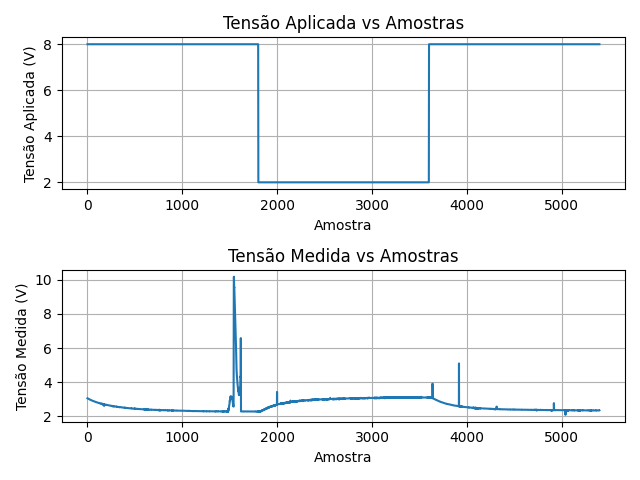
\includegraphics[width=0.75\linewidth]{../identificacao/experimento.png}
    \caption{Curvas de resposta do sistema à aplicação dos degraus.}
    \label{fig:experimento}
\end{figure}

A visualização das curvas expõe a presença de ruído e de fortes pertubações pontuais. Para a continuídade da análise, as primeiras 1620 amostras são descartadas. As curvas resultantes são apresentadas na figura \ref{fig:experimento_valido}.

\begin{figure}[H]
    \centering
    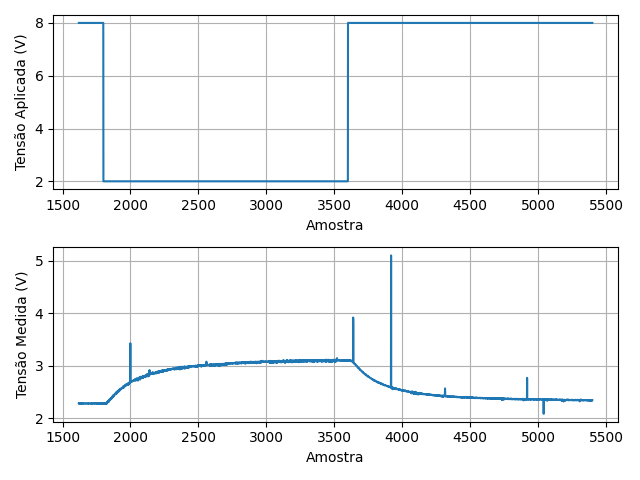
\includegraphics[width=0.75\linewidth]{../identificacao/experimento_valido.png}
    \caption{Curvas de resposta do sistema à aplicação dos degraus, após descarte das amostras iniciais.}
    \label{fig:experimento_valido}
\end{figure}

\section{Identificação do Sistema}

Pelas características térmicas do sistema, no qual a dinâmica da temperatura na planta é estimada muito mais rápida do que a dinâmica da temperatura no sensor, é esperado que o modelo \ref{eq:modelo} seja adequado para representar a dinâmica da planta.

\begin{equation}
    \label{eq:modelo}
    G(s) = \frac{K}{\tau s + 1}
\end{equation}

Para a estimação de valores iniciais para os parâmetros $K$ e $\tau$, a resposta ao primeiro degrau, contida no intervalo $k \in [1800, 3600]$, é utilizada. Então, os parametros são refinados por otimização numérica sobre a resposta a ambos os degraus, implementada pela função \texttt{scipy.optimize.least\_squares}, da biblioteca \texttt{SciPy}. O modelo identificado é apresentado na equação \ref{eq:modelo_identificado}.

\begin{equation}
    \label{eq:modelo_identificado}
    G(s) = \frac{-0.14}{35.77 s + 1}
\end{equation}

A figura \ref{fig:modelo_vs_referencia} apresenta a comparação entre a resposta do modelo identificado e a resposta medida do sistema a ambos os degraus.

\begin{figure}[H]
    \centering
    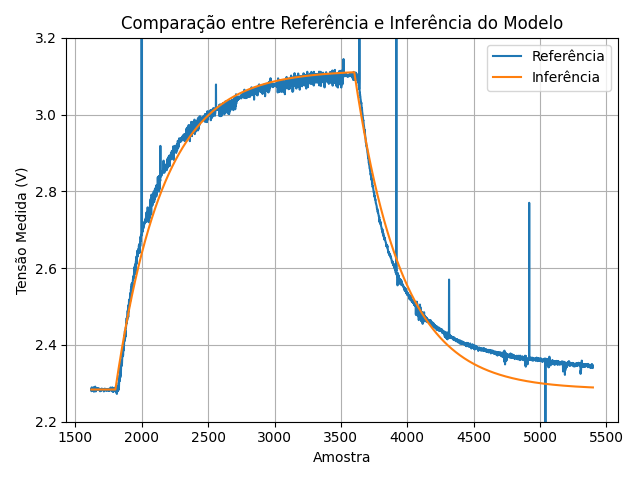
\includegraphics[width=0.75\linewidth]{../identificacao/modelo_vs_referencia.png}
    \caption{Comparação entre a resposta do modelo identificado e a resposta medida do sistema a ambos os degraus.}
    \label{fig:modelo_vs_referencia}
\end{figure}

Por analise visual, o modelo identificado foi considerado adequado.

\section{Filtro Digital}\label{sec:filtro_digital}

Na resposta do sistema, é observada alta incidência de ruído impulsivo, caracterizado por perturbações pontuais de alta amplitude. Para mitigar seus efeitos, um filtro digital de mediana móvel é proposto por \cite{Geoffrine2011}. O tamanho da janela do filtro foi escolhido como $N = 5$ amostras, por experimentação. A figura \ref{fig:mediana} apresenta a comparação entre o sinal bruto e o sinal filtrado.

\begin{figure}[H]
    \centering
    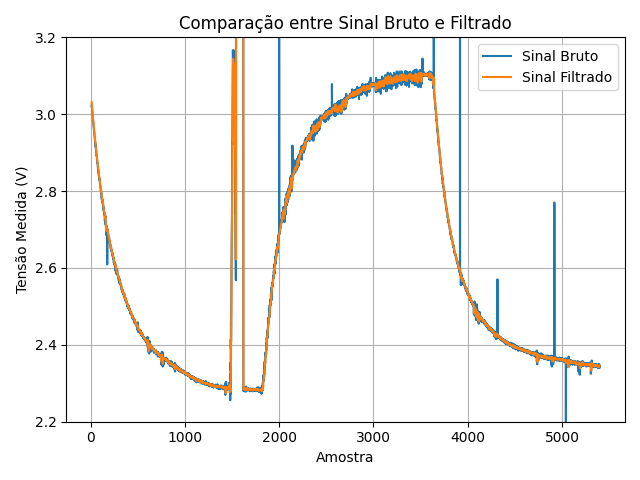
\includegraphics[width=0.75\linewidth]{../filtro/mediana.png}
    \caption{Comparação entre o sinal bruto e o sinal filtrado pelo filtro de mediana móvel.}
    \label{fig:mediana}
\end{figure}

A penalidade deste filtro é a introdução do atraso de $\frac{N - 1}{2} = 2$ amostras, correspondente a $200 ms$. Dada a constante de tempo do sistema, este atraso é considerado aceitável para a aplicação.

A necessidade, ou não, de estender este filtro é dada pela sensibilidade do controlador projetado a ruído\cite{Aguirre2023}. Dados os critérios de aceitação propostos, é esperado que um controlador PI seja suficiente e a extensão, portanto, desnecessária.

Para fins de aprendizado, no entanto, é analizada a justificativa de filtragem para remover componentes de frequências incompatíveis com a dinâmica estimada para o sistema. A fim de preservar a simplicidade do sistema, é escolhido o filtro digital de primeira ordem em \ref{eq:filtro}.

\begin{equation}
    \label{eq:filtro}
    H(z) = \frac{1 - \alpha}{1 - \alpha z^{-1}}
\end{equation}

Neste, $\alpha = e^{-\frac{T_s}{\tau_f}}$, onde $T_s$ é o período de amostragem e $\tau_f = \frac{1}{2 \pi f_c}$ é a constante de tempo do filtro, com $f_c$ a frequência de corte.

Para não atenuar a dinâmica do sistema, $f_c \gg f_\text{mf}$, onde $f_\text{mf} = \frac{1}{2 \pi \tau_\text{mf}}$ é dada pela constante de tempo desejada para o sistema em malha fechada. Conservadoramente, é escolhido $\tau_\text{mf} = 0.5 \tau = 17.89$, o que corresponde a $f_\text{mf} = 0.01\ \text{Hz}$. Pelo teorema de Nyquist-Shannon\cite{Aguirre2023}, $f_c \ll f_\text{Nyquist}$, onde $f_\text{Nyquist} = \frac{1}{2 T_s} = 5\ \text{Hz}$. Destas condições, temos

\begin{equation}
    \label{eq:condicoes_filtro}
    0.01\ \text{Hz} \ll f_c \ll 5\ \text{Hz}
\end{equation}

No espaço logarítmico,

\begin{equation}
    \label{eq:condicoes_filtro_log}
    -2 \ll \log_{10} f_c \ll 0.7
\end{equation}

A fim de maximizar ambas as margens,

\begin{align}
    \log_{10} f_c & = \frac{-2 + 0.7}{2} \\
    \log_{10} f_c & = -0.65 \\
    f_c & = 10^{-0.65} \approx 0.22\ \text{Hz}
\end{align}

Assim, $\tau_f = \frac{1}{2 \pi f_c} \approx 0.72\ s$ e $\alpha = e^{-\frac{T_s}{\tau_f}} \approx 0.88$.

A equação \ref{eq:filtro_sintonizado} apresenta o filtro digital de primeira ordem com os parâmetros calculados.

\begin{equation}
    \label{eq:filtro_sintonizado}
    H(z) = \frac{0.12}{1 - 0.88 z^{-1}}
\end{equation}

Sua implementação em equação de diferenças é dada por

\begin{equation}
    \label{eq:filtro_diferencas}
    y[n] = 0.12 x[n] + 0.88 y[n - 1]
\end{equation}

O filtro digital completo é dado pela equação \ref{eq:filtro_completo}.

\begin{equation}
    \label{eq:filtro_completo}
    \begin{cases}
        x[n] = \text{mediana}(y[n], y[n - 1], y[n - 2], y[n - 3], y[n - 4]) \\
        \hat{y}[n] = 0.12 x[n] + 0.88 \hat{y}[n - 1]
    \end{cases}
\end{equation}

A figura \ref{fig:filtro} apresenta a comparação entre o sinal bruto e o sinal filtrado pelo filtro digital completo.

\begin{figure}[H]
    \centering
    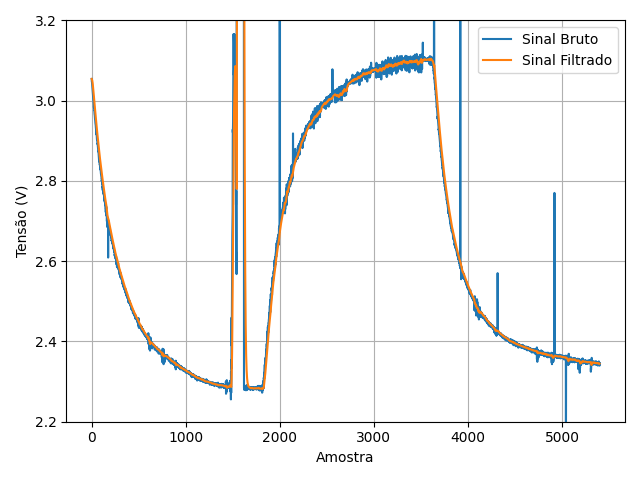
\includegraphics[width=0.75\linewidth]{../filtro/filtro.png}
    \caption{Comparação entre o sinal bruto e o sinal filtrado pelo filtro digital completo.}
    \label{fig:filtro}
\end{figure}

Já a comparação entre os resíduos do sinal bruto, filtrado pela mediana móvel, e filtrado pelo filtro digital completo é apresentada na figura \ref{fig:residuos}. Os resíduos são calculados em relação à resposta do modelo identificado.

\begin{figure}[H]
    \centering
    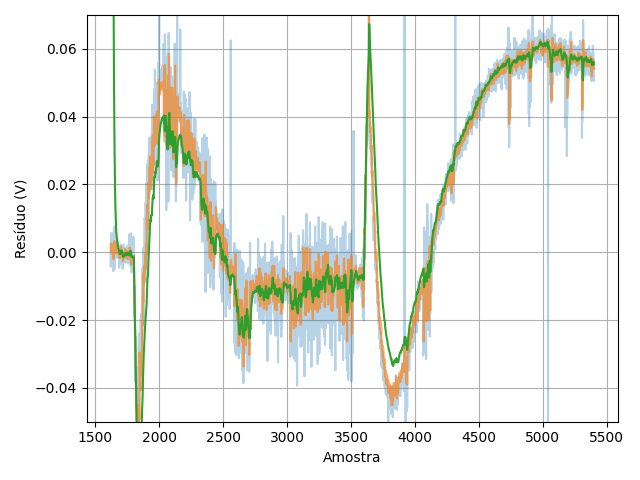
\includegraphics[width=0.75\linewidth]{../filtro/residuos.png}
    \caption{Comparação entre os resíduos do sinal bruto, filtrado pela mediana móvel, e filtrado pelo filtro digital completo. Nesta figura, as curvas azul, laranja e verde correspondem, respectivamente, aos resíduos do sinal bruto, filtrado pela mediana móvel e filtrado pelo filtro digital completo.}
    \label{fig:residuos}
\end{figure}

As curvas em \ref{fig:filtro} indicam preservação da dinâmica do sistema pelo filtro digital, dado que a resposta filtrada segue a resposta do sistema com fidelidade de tendência. Por outro lado, análise visual das curvas de resíduos sugere que o filtro digital atenua os efeitos do ruído de alta frequência melhor do que o filtro de mediana móvel, o que coincide com a expectativa dada pela análise de frequência do sistema e do filtro digital.

Por fim, \ref{fig:validacao} apresenta a comparação entre os sinais bruto e filtrado pela implementação completa do filtro digital no sistema em tempo real, obtidas em um novo experimento, de validação.

\begin{figure}[H]
    \centering
    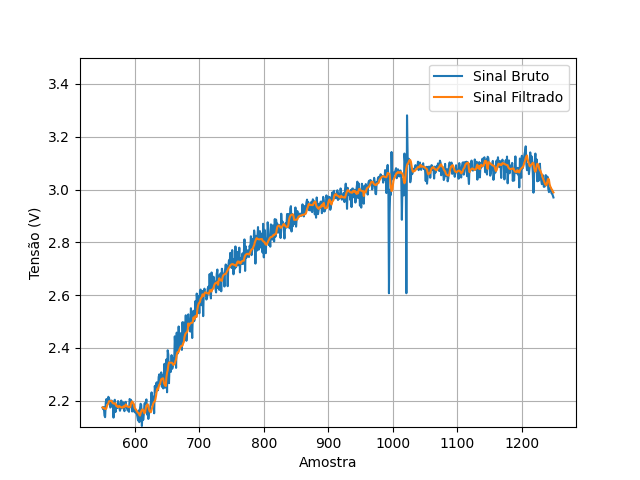
\includegraphics[width=0.75\linewidth]{../filtro/validacao.png}
    \caption{Experimento de validação do filtro digital no sistema em tempo real.}
    \label{fig:validacao}
\end{figure}

A perturbação retangular, de alta amplitude e curta duração, observada na seção anterior à considerada válida, é considerada defeito no sistema de condicionamento do sinal e não tratada neste trabalho.

\section{Controlador}

\subsection{Discretização do Modelo do Sistema}

Discretizado por \textit{Zero-Order Hold}, o modelo do sistema é dado pela equação \ref{eq:modelo_discretizado} \cite{Aguirre2023}.

\begin{equation}
    \label{eq:modelo_discretizado}
    G(z) = \frac{-0.0004z^{-1}}{1 - 0.997z^{-1}}
\end{equation}

Tal função de transferência relaciona a tensão fornecida ao módulo de potência, $u \in \left\{8, 2\right\}\ V$, à tensão de saída do sensor, $y \in \left\{2.0, 0.4\right\}\ V$. A relação entre a tensão de saída do sensor e a temperatura é aproximadamente linear e dada por $T = 10 \left[\frac{^\circ C}{V}\right] \times y\, ^\circ C$. Assim, a função de transferência da entrada em tensão para a saída em temperatura é dada por \ref{eq:modelo_discretizado_temperatura}.

\begin{equation}
    \label{eq:modelo_discretizado_temperatura}
    G(z) = \frac{-0.004z^{-1}}{1 - 0.997z^{-1}}
\end{equation}

\subsection{Modelo do Filtro de Mediana Móvel}

Mesmo que este não seja linear, o filtro de mediana móvel, para as condições deste projeto, pode ser aproximado por um atraso puro de tempo \cite{Geoffrine2011}, conforme \ref{eq:mediana_atraso}.

\begin{equation}
    \label{eq:mediana_atraso}
    M(z) = z^{-2}
\end{equation}

\subsection{Função de Transferência do Sistema em Malha Aberta}

A função de transferência do sistema em malha aberta é dada por \ref{eq:malha_aberta}.

\begin{equation}
    \label{eq:malha_aberta}
    G_\text{aberta}(z) = G(z) H(z) M(z) = \frac{-0.004z^{-1}}{1 - 0.997z^{-1}} \frac{0.12}{1 - 0.88 z^{-1}} z^{-2}
\end{equation}

\subsection{Requisitos e Condições de Estabilidade}

A inequação \ref{eq:condicao_estabilidade} é condição para a estabilidade do sistema em malha fechada \cite{Aguirre2023}.

\begin{align}
    \omega_\text{co} \theta_\text{eq} &\le \Phi_{m_\text{alvo}}  \label{eq:condicao_estabilidade} \\
    \omega_\text{co} \left( \frac{M - 1}{2} + \frac{1}{1 - \alpha} \right) T_s &\le \Phi_{m_\text{alvo}}
\end{align}

Para a constante de tempo alvo definida em \ref{sec:filtro_digital}, a frequência de \textit{crossover} é dada por $f_\text{co} \approx 0.06 \text{Hz}$. Conservadoramente, a margem de fase escolhida é de $\Phi_{m_\text{alvo}} = 45^\circ = \frac{\pi}{4}\ \text{rad}$. Dos valores sintonizados em \ref{sec:filtro_digital},

\begin{equation}
    \label{eq:condicao_estabilidate_satisfeita}
    0.062 \le 0.79
\end{equation}

Assim, a condição de estabilidade é satisfeita, e a margem de fase efetiva do sistema é

\begin{equation}
    \label{eq:margem_fase}
    \Phi_m = 0.79 - 0.062 = 0.73\ \text{rad} \approx 42^\circ
\end{equation}

Abaixo está o excerto atualizado para refletir o projeto do controlador com a trajetória de malha fechada de segunda ordem (filtro de robustez), incluindo a correção dos coeficientes numéricos calculados para $T_s = 0.1$ e $\tau_\text{cl} = 18$.

\subsection{Projeto do Controlador}

Considerada a escolha de aproximar o sistema por um modelo de primeira ordem, e o forte ruído presente nos dados coletados para sua identificação, um controlador baseado em modelo interno é selecionado para o projeto. A principal motivação é sua robustez a imperfeições no modelo do sistema, principalmente quando comparado com controladores baseados em síntese direta \cite{Garcia1982}. Para mitigar a sensibilidade a ruídos em altas frequências e evitar uma ação de controle agressiva, adota-se uma trajetória alvo de malha fechada de segunda ordem.

O modelo em \ref{eq:malha_aberta} é separado em componentes inversível $G_-(z)$ e não inversível $G_+(z)$, tal que

\begin{align}
    G_-(z) & = \frac{-0.004z^{-1}}{1 - 0.997z^{-1}} \\
    G_+(z) & = \frac{0.12}{1 - 0.88 z^{-1}} z^{-2}
\end{align}

O controlador ideal é obtido pela aplicação de um filtro de robustez de segunda ordem $f(z) = \frac{(1 - p)^2}{(1 - p z^{-1})^2}$, com $p = e^{-\frac{T_s}{\tau_\text{cl}}} \approx 0.9945$ -- em \ref{sec:filtro_digital}, é definido $\tau_\text{cl} = \frac{\tau}{2}$, à inversa do componente inversível do sistema. Este é dado por \ref{eq:controlador_ideal}.

\begin{equation}
    \label{eq:controlador_ideal}
    Q(z) = G_-^{-1}(z) f(z) = \frac{1 - 0.997z^{-1}}{-0.004z^{-1}} \frac{(1 - p)^2}{(1 - p z^{-1})^2}
\end{equation}

Com este, o controlador implementável é dado por \ref{eq:controlador_implementavel}.

\begin{align}
    C(z) & = \frac{Q(z)}{1 - Q(z) G(z)} \\
    C(z) & = \frac{-0.008 + 0.014z^{-1} - 0.007z^{-2}}{1 - 2.9z^{-1} + 2.74z^{-2} - 0.87z^{-3}} \label{eq:controlador_implementavel}
\end{align}

Sua implementação em equação de diferenças é dada por \ref{eq:controlador_diferencas}.

\begin{align}
    u[n] =\ & -0.008\, e[n] + 0.014\, e[n-1] - 0.007\, e[n-2] \notag \\
           & + 2.9\, u[n-1] - 2.74\, u[n-2] + 0.87\, u[n-3]
    \label{eq:controlador_diferencas}
\end{align}

\subsection{Função de Transferência de Malha Fechada}

A função de transferência de malha fechada é dada por \ref{eq:malha_fechada}.

\begin{equation}
    \label{eq:malha_fechada}
    G_\text{fechada}(z) = \frac{G(z) C(z)}{1 + G(z) H(z) M(z) C(z)}
\end{equation}

Para os modelos identificados, assumindo $M(z) \approx 1$ para $z \to 1$, a dinâmica nominal fechada resulta em \ref{eq:malha_fechada_calculada}.

\begin{equation}
    \label{eq:malha_fechada_calculada}
    T(z) = \frac{- 0.0001 z^{-2} + 0.0001 z^{-3}}{1 - 3.9z^{-1} + 5.6z^{-2} - 3.6z^{-3} + 0.9z^{-4}}
\end{equation}

\subsubsection{Polos e Zeros}



\bibliography{bibliografia}

\end{document}
